\documentclass[tikz, border=10pt]{standalone}
\usetikzlibrary{calc, angles, quotes}
\begin{document}
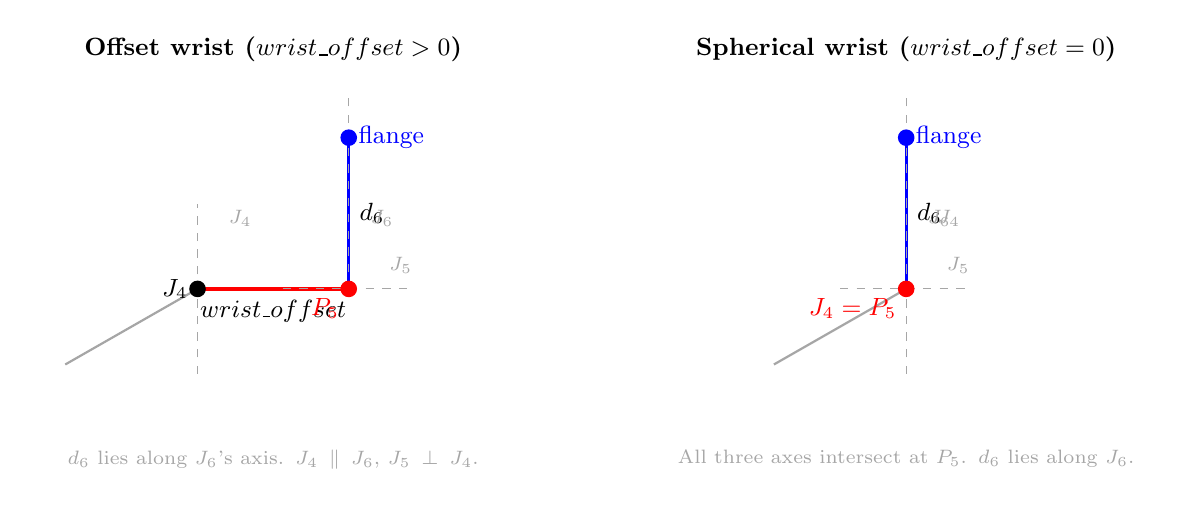
\begin{tikzpicture}[scale=1.2, >=stealth]

    % ==========================================================
    % LEFT PANEL: OFFSET WRIST (wrist_offset > 0)
    % ==========================================================
    \begin{scope}[shift={(0,0)}]

        % Key points. J4 at origin, P5 horizontally offset, flange above P5.
        \coordinate (J4) at (0, 0);
        \coordinate (P5) at (1.6, 0);          % horizontal offset from J4
        \coordinate (F)  at (1.6, 1.6);        % vertical offset from P5 (along J6 axis)

        % Forearm (arrives at J4 from lower left)
        \draw[gray!70, thick] (-1.4, -0.8) -- (J4);

        % Wrist-1 link (J4 to P5): horizontal
        \draw[red, very thick] (J4) -- (P5)
              node[midway, below, black, font=\small] {\(wrist\_offset\)};

        % Flange offset (P5 to F): vertical, along J6 axis
        \draw[blue, very thick] (P5) -- (F)
              node[midway, right, black, font=\small] {\(d_6\)};

        % --- Joint axes ---
        % J4 axis: vertical
        \draw[gray!70, dashed] ($ (J4) + (0, -0.9) $) -- ($ (J4) + (0, 0.9) $);
        \node[gray!70, font=\scriptsize] at ($ (J4) + (0.45, 0.75) $) {\(J_4\)};

        % J5 axis: horizontal (perpendicular to J4)
        \draw[gray!70, dashed] ($ (P5) + (-0.7, 0) $) -- ($ (P5) + (0.7, 0) $);
        \node[gray!70, font=\scriptsize] at ($ (P5) + (0.55, 0.25) $) {\(J_5\)};

        % J6 axis: vertical, through P5 and the flange
        \draw[gray!70, dashed] ($ (P5) + (0, 0) $) -- ($ (F) + (0, 0.5) $);
        \node[gray!70, font=\scriptsize] at ($ (P5) + (0.35, 0.75) $) {\(J_6\)};

        % Points
        \fill (J4) circle (2.5pt) node[left, font=\small] {\(J_4\)};
        \fill[red] (P5) circle (2.5pt) node[below left, font=\small] {\(P_5\)};
        \fill[blue] (F) circle (2.5pt) node[right, font=\small] {flange};

        % Title
        \node[above, font=\small\bfseries] at (0.8, 2.3) {Offset wrist (\(wrist\_offset > 0\))};

        % Note
        \node[below, font=\scriptsize, gray!70, text width=6cm, align=center]
              at (0.8, -1.6) {\(d_6\) lies along \(J_6\)'s axis. \(J_4 \parallel J_6\), \(J_5 \perp J_4\).};

    \end{scope}

    % ==========================================================
    % RIGHT PANEL: SPHERICAL WRIST (wrist_offset = 0)
    % ==========================================================
    \begin{scope}[shift={(7.5, 0)}]

        \coordinate (J4P5) at (0, 0);
        \coordinate (F) at (0, 1.6);            % vertical, along J6 axis

        % Forearm
        \draw[gray!70, thick] (-1.4, -0.8) -- (J4P5);

        % Flange offset: vertical
        \draw[blue, very thick] (J4P5) -- (F)
              node[midway, right, black, font=\small] {\(d_6\)};

        % --- Joint axes: all pass through J4P5 ---
        % J4 axis: vertical
        \draw[gray!70, dashed] ($ (J4P5) + (0, -0.9) $) -- ($ (J4P5) + (0, 0.9) $);
        \node[gray!70, font=\scriptsize] at ($ (J4P5) + (0.45, 0.75) $) {\(J_4\)};

        % J5 axis: horizontal
        \draw[gray!70, dashed] ($ (J4P5) + (-0.7, 0) $) -- ($ (J4P5) + (0.7, 0) $);
        \node[gray!70, font=\scriptsize] at ($ (J4P5) + (0.55, 0.25) $) {\(J_5\)};

        % J6 axis: vertical (same as J4)
        \draw[gray!70, dashed] ($ (J4P5) + (0, 0) $) -- ($ (F) + (0, 0.5) $);
        \node[gray!70, font=\scriptsize] at ($ (J4P5) + (0.35, 0.75) $) {\(J_6\)};

        % Points
        \fill[red] (J4P5) circle (2.5pt) node[below left, font=\small] {\(J_4 = P_5\)};
        \fill[blue] (F) circle (2.5pt) node[right, font=\small] {flange};

        % Title
        \node[above, font=\small\bfseries] at (0.0, 2.3) {Spherical wrist (\(wrist\_offset = 0\))};

        % Note
        \node[below, font=\scriptsize, gray!70, text width=6cm, align=center]
              at (0.0, -1.6) {All three axes intersect at \(P_5\). \(d_6\) lies along \(J_6\).};

    \end{scope}

\end{tikzpicture}
\end{document}